\documentclass[a4paper,12pt]{article}
%%% Работа с русским языком % для pdfLatex
\usepackage{cmap}					% поиск в~PDF
\usepackage{mathtext} 				% русские буквы в~фомулах
\usepackage[T2A]{fontenc}			% кодировка
\usepackage[utf8]{inputenc}			% кодировка исходного текста
\usepackage[english,russian]{babel}	% локализация и переносы
\usepackage{indentfirst} 			% отступ 1 абзаца

%%% Работа с русским языком % для XeLatex
%\usepackage[english,russian]{babel}   %% загружает пакет многоязыковой вёрстки
%\usepackage{fontspec}      %% подготавливает загрузку шрифтов Open Type, True Type и др.
%\defaultfontfeatures{Ligatures={TeX},Renderer=Basic}  %% свойства шрифтов по умолчанию
%\setmainfont[Ligatures={TeX,Historic}]{Times New Roman} %% задаёт основной шрифт документа
%\setsansfont{Comic Sans MS}                    %% задаёт шрифт без засечек
%\setmonofont{Courier New}
%\usepackage{indentfirst}
%\frenchspacing

%%% Дополнительная работа с математикой
\usepackage{amsfonts,amssymb,amsthm,mathtools}
\usepackage{amsmath}
\usepackage{icomma} % "Умная" запятая: $0,2$ --- число, $0, 2$ --- перечисление
\usepackage{upgreek}

%% Номера формул
%\mathtoolsset{showonlyrefs=true} % Показывать номера только у тех формул, на которые есть \eqref{} в~тексте.

%%% Страница
\usepackage{extsizes} % Возможность сделать 14-й шрифт

%% Шрифты
\usepackage{euscript}	 % Шрифт Евклид
\usepackage{mathrsfs} % Красивый матшрифт

%% Свои команды
\DeclareMathOperator{\sgn}{\mathop{sgn}} % создание новой конанды \sgn (типо как \sin)
\usepackage{csquotes} % ещё одна штука для цитат
\newcommand{\pd}[2]{\ensuremath{\cfrac{\partial #1}{\partial #2}}} % частная производная
\newcommand{\abs}[1]{\ensuremath{\left|#1\right|}} % модуль
\renewcommand{\phi}{\ensuremath{\varphi}} % греческая фи
\newcommand{\pogk}[1]{\!\left(\cfrac{\sigma_{#1}}{#1}\right)^{\!\!\!2}\!} % для погрешностей

% Ссылки
\usepackage{color} % подключить пакет color
% выбрать цвета
\definecolor{BlueGreen}{RGB}{49,152,255}
\definecolor{Violet}{RGB}{120,80,120}
% назначить цвета при подключении hyperref
\usepackage[unicode, colorlinks, urlcolor=blue, linkcolor=blue, pagecolor=blue, citecolor=blue]{hyperref} %синие ссылки
%\usepackage[unicode, colorlinks, urlcolor=black, linkcolor=black, pagecolor=black, citecolor=black]{hyperref} % для печати (отключить верхний!)


%% Перенос знаков в~формулах (по Львовскому)
\newcommand*{\hm}[1]{#1\nobreak\discretionary{}
	{\hbox{$\mathsurround=0pt #1$}}{}}

%%% Работа с картинками
\usepackage{graphicx}  % Для вставки рисунков
\graphicspath{{images/}{images2/}}  % папки с картинками
\setlength\fboxsep{3pt} % Отступ рамки \fbox{} от рисунка
\setlength\fboxrule{1pt} % Толщина линий рамки \fbox{}
\usepackage{wrapfig} % Обтекание рисунков и таблиц текстом
\usepackage{multicol}

%%% Работа с таблицами
\usepackage{array,tabularx,tabulary,booktabs} % Дополнительная работа с таблицами
\usepackage{longtable}  % Длинные таблицы
\usepackage{multirow} % Слияние строк в~таблице
\usepackage{caption}
\captionsetup{labelsep=period, labelfont=bf}

%%% Оформление
\usepackage{indentfirst} % Красная строка
%\setlength{\parskip}{0.3cm} % отступы между абзацами
%%% Название разделов
\usepackage{titlesec}
\titlelabel{\thetitle.\quad}
\renewcommand{\figurename}{\textbf{Рис.}}		%Чтобы вместо figure под рисунками писал "рис"
\renewcommand{\tablename}{\textbf{Таблица}}		%Чтобы вместо table над таблицами писал Таблица

%%% Теоремы
\theoremstyle{plain} % Это стиль по умолчанию, его можно не переопределять.
\newtheorem{theorem}{Теорема}[section]
\newtheorem{proposition}[theorem]{Утверждение}

\theoremstyle{definition} % "Определение"
\newtheorem{definition}{Определение}[section]
\newtheorem{corollary}{Следствие}[theorem]
\newtheorem{problem}{Задача}[section]

\theoremstyle{remark} % "Примечание"
\newtheorem*{nonum}{Решение}
\newtheorem{zamech}{Замечание}[theorem]

%%% Правильные мат. символы для русского языка
\renewcommand{\epsilon}{\ensuremath{\varepsilon}}
\renewcommand{\phi}{\ensuremath{\varphi}}
\renewcommand{\kappa}{\ensuremath{\varkappa}}
\renewcommand{\le}{\ensuremath{\leqslant}}
\renewcommand{\leq}{\ensuremath{\leqslant}}
\renewcommand{\ge}{\ensuremath{\geqslant}}
\renewcommand{\geq}{\ensuremath{\geqslant}}
\renewcommand{\emptyset}{\varnothing}

\usepackage{bm} %жирный греческий шрифт
%\usepackage{ulem}

\graphicspath{{images}}

\title{Laba 2.2.6}
\author{Георгий Демьянов}
\date{today}
\usepackage[left=1.27cm,right=1.27cm,top=1.27cm,bottom=2cm]{geometry}

\begin{document} 
\begin{titlepage}
\begin{center} 
 
\large Московский физико-технический институт\\
Факультет молекулярной и химической физики\\
\vspace{7cm}
\huge Лабораторная работа №2.2.6\\
\textbf{\Large <<Определение энергии активации по температурной зависимости вязкости жидкости>>}\\
\end{center} 

\vspace{7.5cm}
{\par \raggedleft \large \emph{Выполнил:}\\ студент 1 курса\\ 642 группы ФМХФ\\ Демьянов Георгий\\ Сергеевич \par}
\begin{center}
\vfill Москва 2017
\end{center}
\end{titlepage}

\newpage
\setcounter{page}{2}

\begin{center}
	\vspace{0.5cm}{\parbox{16cm}{\small{\centering{\textbf{Аннотация}\\
					\hspace{0.6cm} В этом отчёте изложены результаты выполнения лабораторной работы «Определение энергии активации по температурной зависимости вязкости жидкости». С помощью термостата изменялась температура в ёмкости с глицерином. При нескольких значениях температур в ёмкость бросали шарики из стекла и жести. Измеряли время их падения, из чего находили скорость движения шариков в глицерине. Отсюда получили значение энергии активации глицерина.
				}}}}
\end{center}

\textbf{\emph{Цель работы:}} расчет энергии активации глицерина.
\section{Теоретическое введение}
В отличие от твердых тел, жидкости обладают «рыхлой» структурой. В них имеются свободные места — «дырки», благодаря чему
молекулы могут перемещаться, покидая свое место и занимая одну
из соседних дырок. Таким образом, молекулы медленно перемещаются внутри жидкости, пребывая часть времени около определенных
мест равновесия и образуя картину меняющейся со временем пространственной решетки. На современном языке принято говорить, что в жидкости присутствует ближний, но не дальний порядок,
расположение молекул упорядочено в небольших объемах, но порядок перестает замечаться при увеличении расстояния.

Как уже отмечалось, для того чтобы перейти в новое состояние,
молекула должна преодолеть участки с большой потенциальной энергией, превышающей среднюю тепловую энергию молекул. Для этого
тепловая энергия молекул должна — вследствие флуктуации — увеличиться на некоторую величину $W$ , называемую энергией активации.
Вследствие этого переходы молекул из одного положения равновесия в другое происходят сравнительно редко и тем реже, чем больше
энергия активации.

Отмеченный характер движения молекул объясняет как медленность диффузии в жидкостях, так и большую (по сравнению с газами) их вязкость. В газах вязкость объясняется происходящим при
тепловом движении молекул переносом количества направленного
движения. В жидкостях такие переходы существенно замедлены. Количество молекул, имеющих энергии больше $W$, в соответствии с формулой Больцмана экспоненциально зависит от $W$. Температурная зависимость вязкости жидкости выражается формулой
\begin{equation}
\eta = A e^{W/kT}
\label{Eq:eta}
\end{equation}

Из формулы \eqref{Eq:eta} следует, что вязкость жидкости при повышении температуры должна резко уменьшаться. Если отложить на графике логарифм вязкости $\ln\eta$ в зависимости от $1/T$ , то согласно \eqref{Eq:eta} должна получиться прямая линия, по угловому коэффициенту которой можно
определить энергию активации молекулы $W$ исследуемой жидкости.
Экспериментальные исследования показывают, что в небольших температурных интервалах эта формула неплохо описывает изменение
вязкости с температурой. При увеличении температурного интервала согласие получается плохим, что представляется вполне естественным, поскольку формула \eqref{Eq:eta} выведена при очень грубых предположениях.
Для исследования температурной зависимости вязкости жидкости в данной работе используется метод Стокса, основанный на измерении скорости свободного падения шарика в жидкости. Суть его
заключается в следующем.


На всякое тело, двигающееся в вязкой жидкости, действует сила сопротивления. В общем случае величина этой силы зависит от многих факторов: от вязкости жидкости, от формы тела, от характера
обтекания и т. д. Стоксом было получено строгое решение задачи
о ламинарном обтекании шарика безграничной жидкостью. В этом
случае сила сопротивления $F$ определяется формулой
\begin{equation}
F=6\pi \eta r v,
\label{Eq:stoks}
\end{equation}
где $\eta$ --- вязкость жидкости, $v$ --- скорость шарика, $r$ --- его радиус.

При свободном падении шарика в вязкой жидкости на шарик действуют три силы: сила тяжести, архимедова сила и сила
вязкости, зависящая от скорости.

Найдем уравнение движения шарика в жидкости. По второму закону Ньютона:
\begin{equation}
Vg(\rho-\rho_{\text{ж}})-6\pi \eta r v=V\rho \cfrac{dv}{dt},
\label{Eq:newton}
\end{equation}
где $V$ --- объем шарика, $\rho$ --- его плотность, $\rho_{\text{ж}}$ --- плотность жидкости,
$g$ --- ускорение свободного падения. Решая это уравнение, найдем
\begin{equation}
v(t) = v_{\text{уст}}-[v_{\text{уст}}-v(0)]e^{-t/\tau}
\label{Eq:skorost}
\end{equation}
В формуле \eqref{Eq:skorost} приняты обозначения: $v(0)$ --- скорость шарика в момент начала его движения в жидкости,
\begin{equation}
	v_{\text{уст}}=\cfrac{2}{9}\,gr^2\cfrac{\rho-\rho_{\text{ж}}}{\eta}, \qquad \tau=\cfrac{2r^2\rho}{9\eta}
	\label{Eq:obozn}
\end{equation}

Как видно из \eqref{Eq:skorost}, скорость шарика экспоненциально приближается к установившейся скорости $v_{\text{уст}}$. Установление скорости определяется величиной $\tau$, имеющей размерность времени и называющейся
временем релаксации. Если время падения в несколько раз больше
времени релаксации, процесс установления скорости можно считать
закончившимся.

Измеряя на опыте установившуюся скорость падения шариков
$v_{\text{уст}}$ и величины $r$, $\rho$, $\rho_{\text{ж}}$, можно определить вязкость жидкости по
формуле, следующей из \eqref{Eq:obozn}
\begin{equation}
\eta=\cfrac{2}{9}\,gr^2\cfrac{\rho-\rho_{\text{ж}}}{v_{\text{уст}}}.
\label{eta_v}
\end{equation}

Полезно также найти путь релаксации S, путем интегрирования \eqref{Eq:skorost}, полагая $v(0)=0$:
\begin{equation}
S=v_{\text{уст}}\tau (t/\tau-1+e^{-t/\tau}) \Rightarrow S \gg \tau v_{\text{уст}}, t \gg \tau.
\label{Eq:s}
\end{equation}

Теория взята из \cite{Gladun:PrakTermodin}~--~c. 74--76.
\section{Экспериментальная установка}
Схема прибора (в разрезе) показана
на рис. \ref{fig:ust}.

Для измерений используется
стеклянный цилиндрический сосуд В, наполненный исследуемой жидкостью (глицерин). На стенках сосуда нанесены две метки на некотором расстоянии друг от друга. Верхняя метка располагаться ниже уровня жидкости с таким расчётом, чтобы скорость
шарика к моменту прохождения этой метки успевала установиться.

Сам сосуд В помещён в рубашку Б, омываемую водой из термостата.
При работающем термостате температура воды в рубашке Б, а потому и температура жидкости 12 равна температуре воды в термостате.

Радиусы шариков измеряются горизонтальным компаратором
или микроскопом.

Ванна представляет собой емкость из нержавеющей стали, установленную в наружный кожух.
В блоке терморегулирования расположены: насос для обеспечения перемешивания рабочей жидкости и перекачки её во внешний
контур, нагреватель, датчик температуры, датчик уровня жидкости,
элементы управления и индикации, необходимые для надёжной работы.

\begin{figure}[h!]
	\centering
	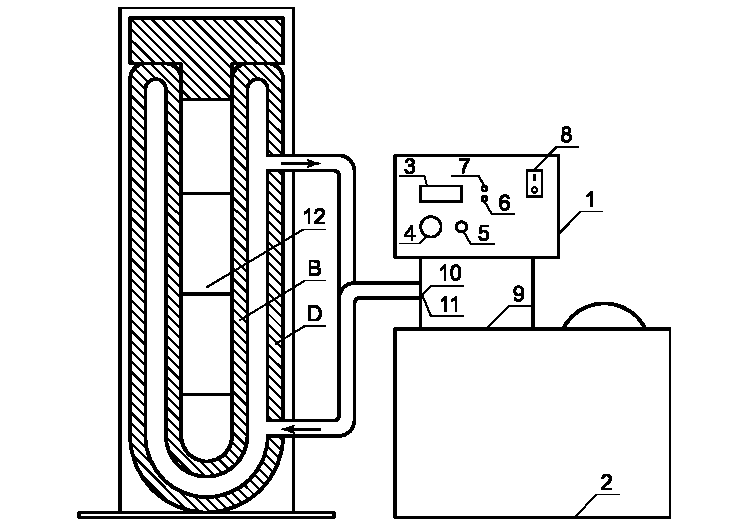
\includegraphics[width=0.8\linewidth]{ust}
	\caption{Установка для определения коэффициента вязкости жидкости\\
	1 --- блок терморегулирования;\\
	2 --- ванна;\\
	3 --- индикаторное табло;\\
	4 --- ручка установки температуры;\\
	5 --- кнопка переключения режимов установки/контроля температуры;\\
	6 --- индикатор уровня жидкости;\\
	7 --- индикатор включения нагревателя;\\
	8 --- сетевой выключатель прибора;\\
	9 --- крышка;\\
	10 --- входной и выходной патрубки насоса;\\
	11 --- входной и выходной патрубки теплообменника\\
	12 --- жидкость
	}
	\label{fig:ust}
\end{figure}

Описание взято из \cite{Gladun:PrakTermodin}~--~c. 76.

\section{Обработка результатов измерений}
\subsection{Обработка результатов}

Будем записывать температуру, которую нам показывает термостат. Также, измерим диаметр каждого шарика, запишем материал шарика. Измерим время, за которое шарик будет проходить от одной метки на емкости с глицерином до другой. Весь эксперимент, кроме первого измерения, был отснят на камеру с частотой 60 кадров/с. С помощью графика $\rho_{\text{ж}}(T)$ найдем значение плотности глицерина (рис. \ref{ro_graph}). Измерим расстояния между метками с помощью линейки. Значения плотности материала шарика возьмем из табличных данных.

\begin{figure}%{r}{0.3\linewidth}
	\centering
	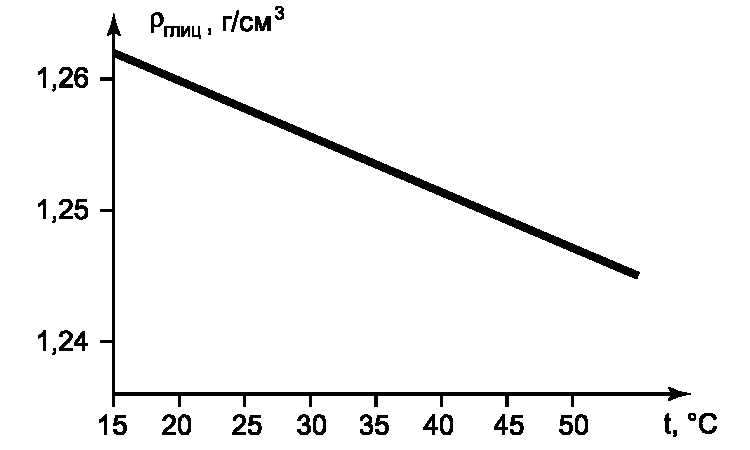
\includegraphics[width=0.7\linewidth]{ro_graph}
	\caption{Зависимость плотности глицерина от температуры}
	\label{ro_graph}
\end{figure}

Полученные данные занесем в таблицу \ref{Tab:tab_exp}.
 
\begin{table}%FIXME поправить таблицы
	\centering
	\begin{tabular}{c}
	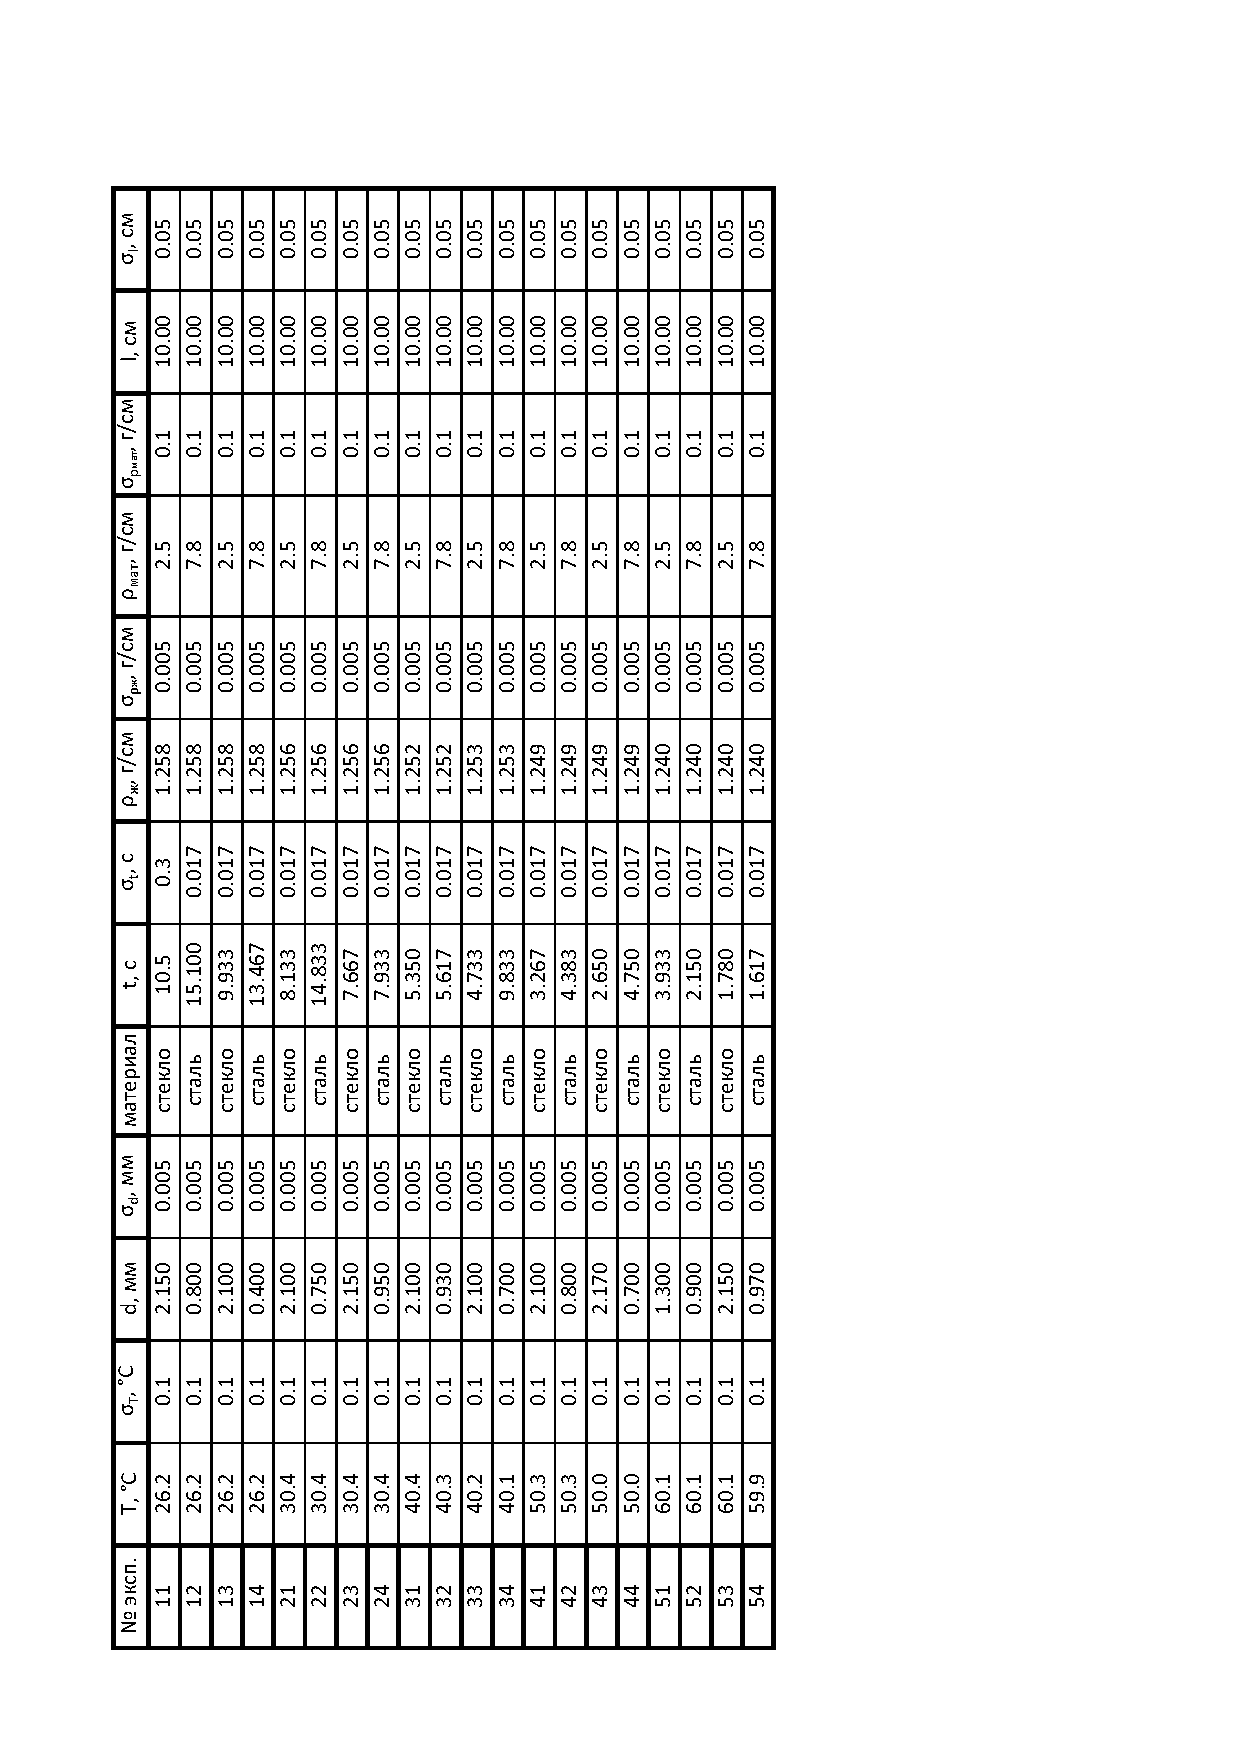
\includegraphics[height=0.9\textheight]{tabel_exp}\\
	\end{tabular}
	\caption{Табличные данные и значения, полученные при проведении эксперимента}
	\label{Tab:tab_exp}
\end{table}

Рассчитаем скорость движения шарика и её погрешность по формулам
\begin{equation}
v_{\text{уст}}=\cfrac{l}{t}, \qquad \pogk{v_{\text{уст}}}=\pogk{l}+\pogk{t}.
\end{equation}
Далее, пользуясь \eqref{eta_v}, рассчитаем значения $\eta$, а погрешность найдем так:
$$
\pogk{\eta}=4\pogk{r}+\pogk{\rho-\rho_{\text{ж}}}+\pogk{v_{\text{уст}}}, \qquad \sigma_{\rho-\rho_{\text{ж}}}^2=\sigma_{\rho}^2+\sigma_{\rho_{\text{ж}}}^2.
$$
Полученные значения внесем в таблицу \ref{Tab:eta_v}.
\begin{table} %FIXME поправить таблицы
	\centering
	\begin{tabular}{c}
		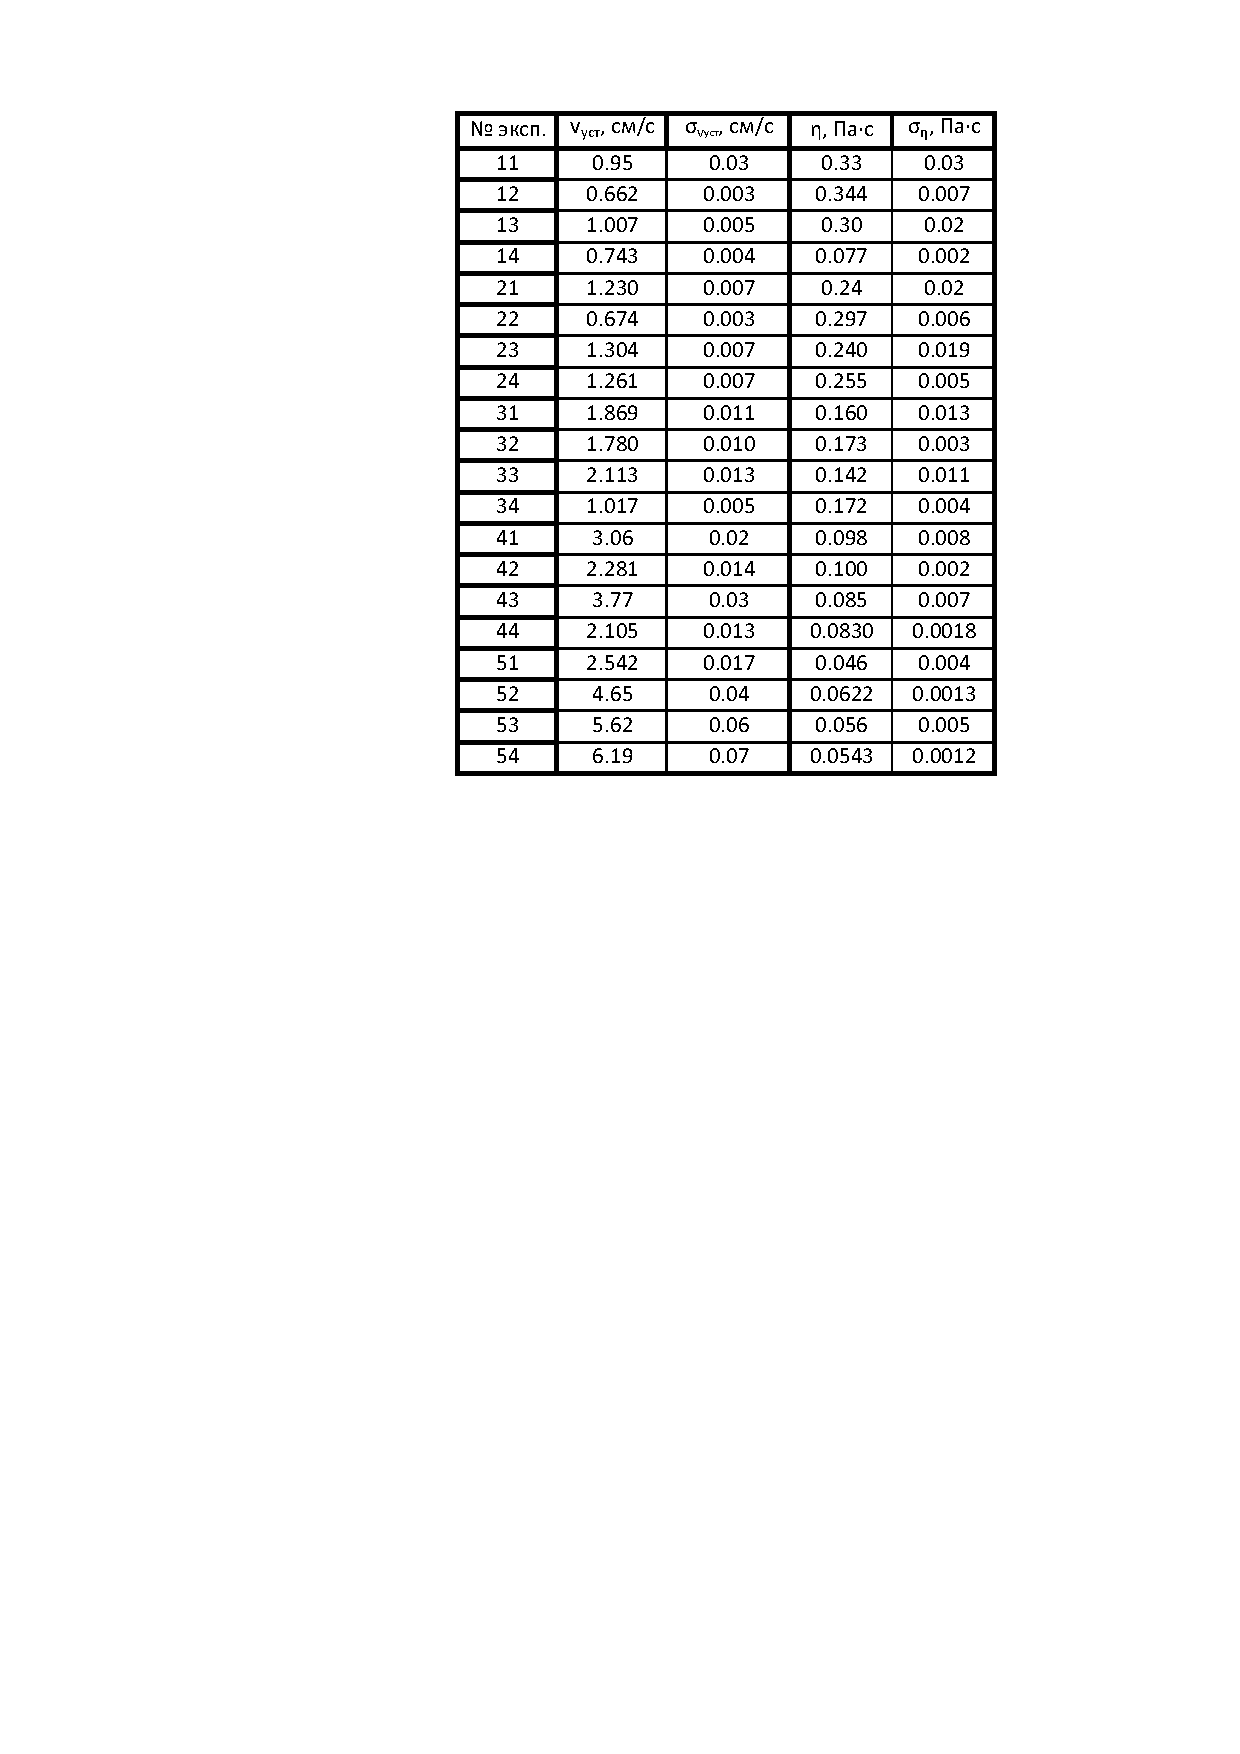
\includegraphics[height=0.4\textheight]{tab_2}\\
	\end{tabular}
	\caption{Значения $v_{\text{уст}}$ и $\eta$}
	\label{Tab:eta_v}
\end{table}

Оценим значения числа Re=$\frac{\rho_{\text{ж}} v r}{\eta}$, $\tau$, $S$ по формулам \eqref{Eq:obozn}, \eqref{Eq:s} и занесем в таблицу \ref{Tab:Re}.
\begin{table} %FIXME поправить таблицы
	\centering
	\begin{tabular}{c}
		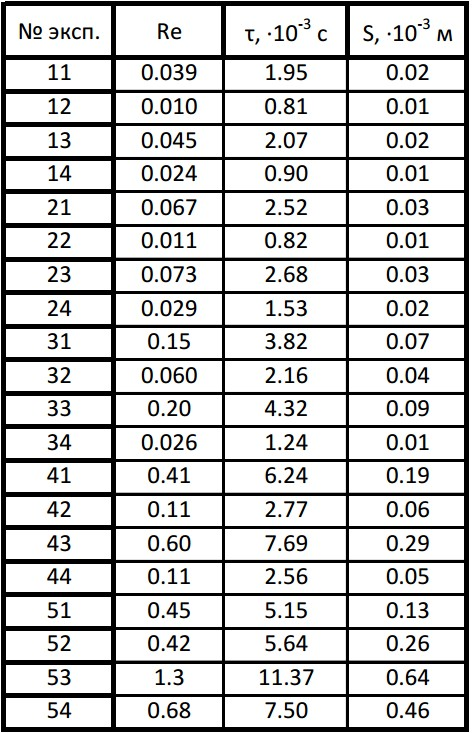
\includegraphics[height=0.4\textheight]{exp_re}\\
	\end{tabular}
	\caption{Значения Re, $\tau$ и $S$}
	\label{Tab:Re}
\end{table}

Значения чисел Re $\sim$ 0.5. Это свидетельствует о ламинарном течении, что действительно позволяет применить формулу Стокса. Малость значений времени и пути релаксации говорит о справедливости наших приближений, т.е. что к моменту прохождения метки старта скорость шарика приобретает установившийся характер.

Нанесём на график экспериментальные точки $\ln \eta(\frac{1}{T})$ и проведём по ним прямую методом наименьших квадратов (МНК, рис. \ref{Fig:graph}). Тогда коэффициент наклона прямой есть $W/k$.

Эксперимент 14 пришлось отбросить, т.к. значение слишком сильно отличается от остальных.

\begin{figure}
	\centering
	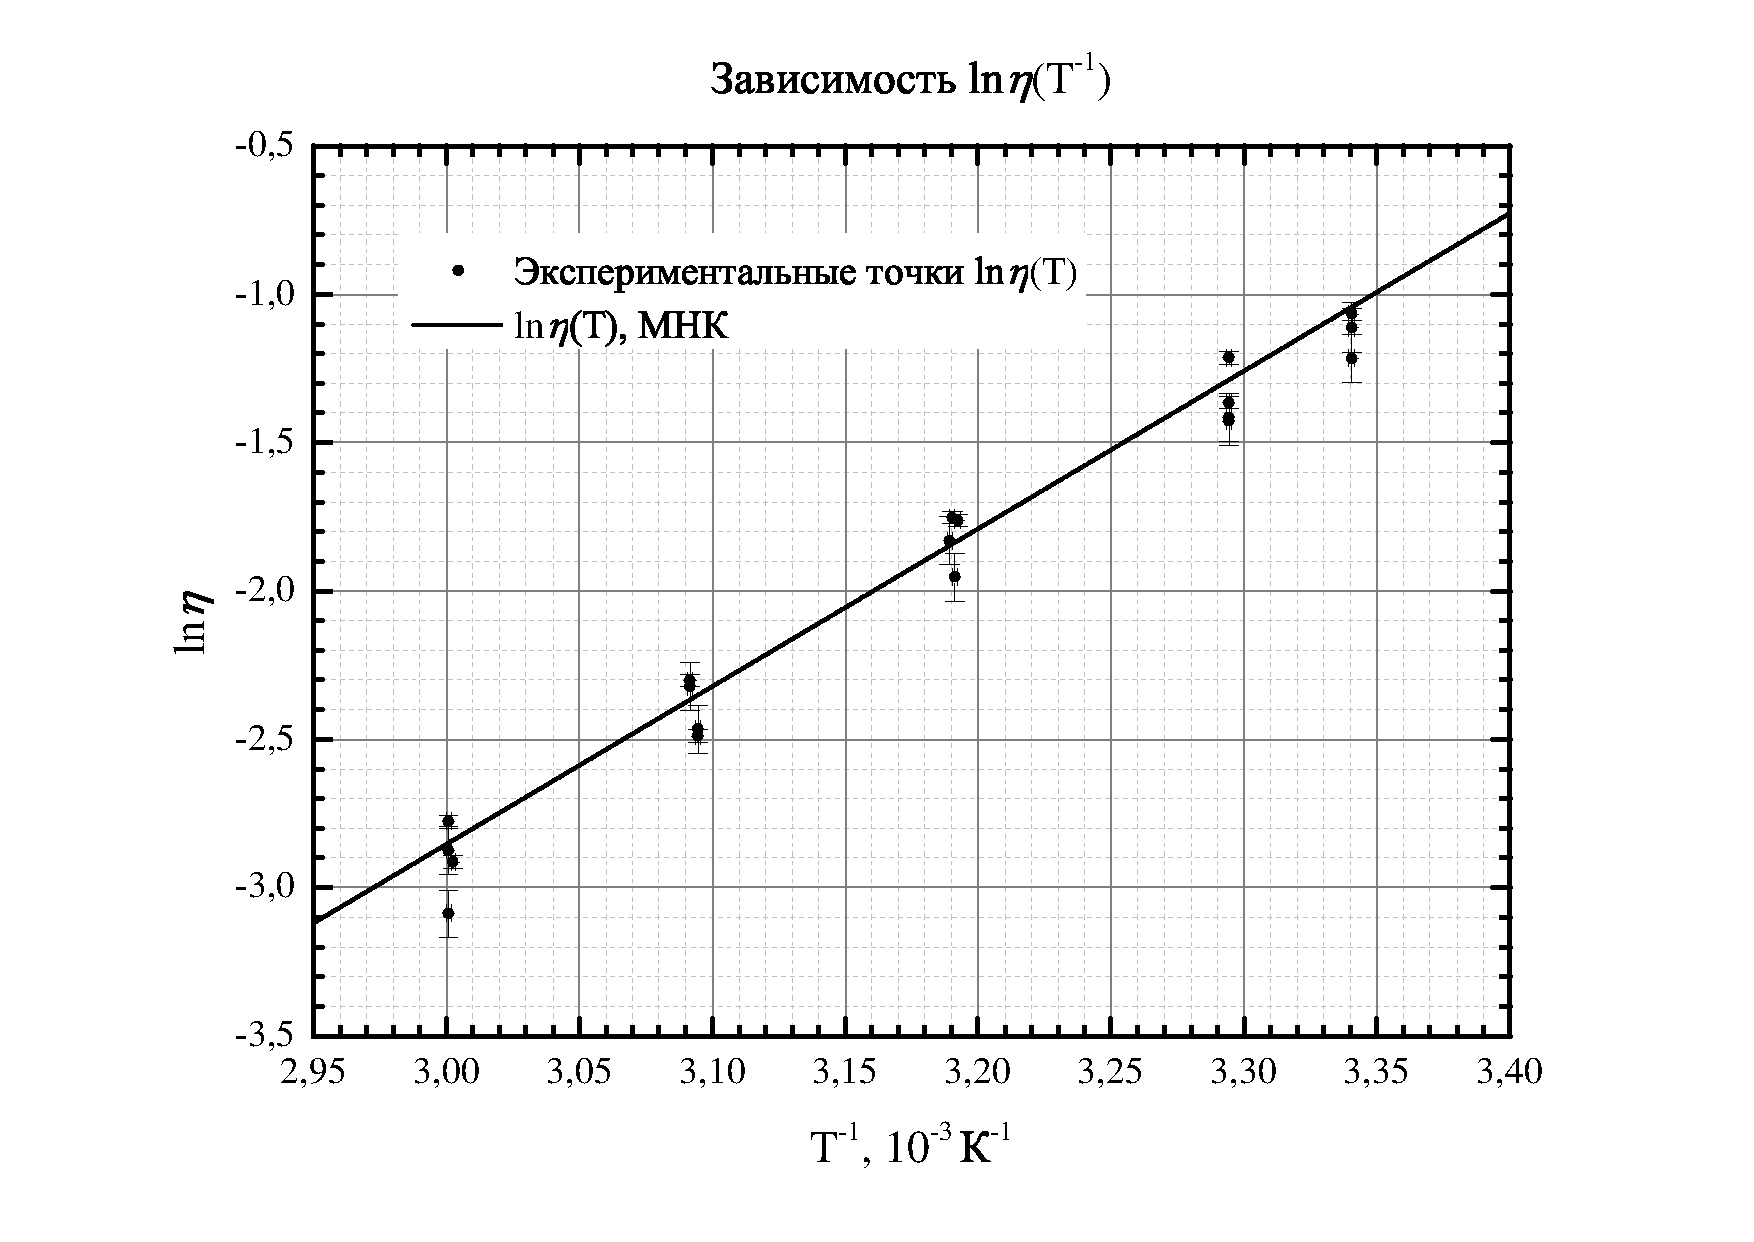
\includegraphics[width=0.8\linewidth]{graph}
	\caption{Зависимость $\ln \eta(\frac{1}{T})$}
	\label{Fig:graph}
\end{figure}

Из МНК, получим:
\begin{equation}
\frac{W}{k}=(532\pm6)\cdot 10 \text{ К}\Rightarrow W=(7.34\pm0.08)\cdot 10^{-20} \text{ Дж}=\underline{0.458\pm0.005 \text{ эВ}}.
\end{equation}

\subsection{Сравнение значения с другими данными}
В работе <<Измерение вязкости жидкостей по затуханию колебаний камертона>> \cite{Stat:Agafon} было получено следующее значение энергии активации:
$$
W = (7.247\pm0.017)\cdot 10^{-20} \text{ Дж} = (0.4529\pm 0.0011) \text{ эВ}.
$$
Полученное в данной лабораторной работе значение  находится в достаточном согласии с этим значением (отличие на 1.1 \%).

В справочнике Григорьева <<Физические величины>> (таблица 16.17, \cite{Grigoriev:Fiz_Velichini}) приведены значения вязкости глицерина (таблица \ref{Tab:tab_dann}),
\begin{table} %FIXME поправить таблицы
	\centering
	\begin{tabular}{c}
		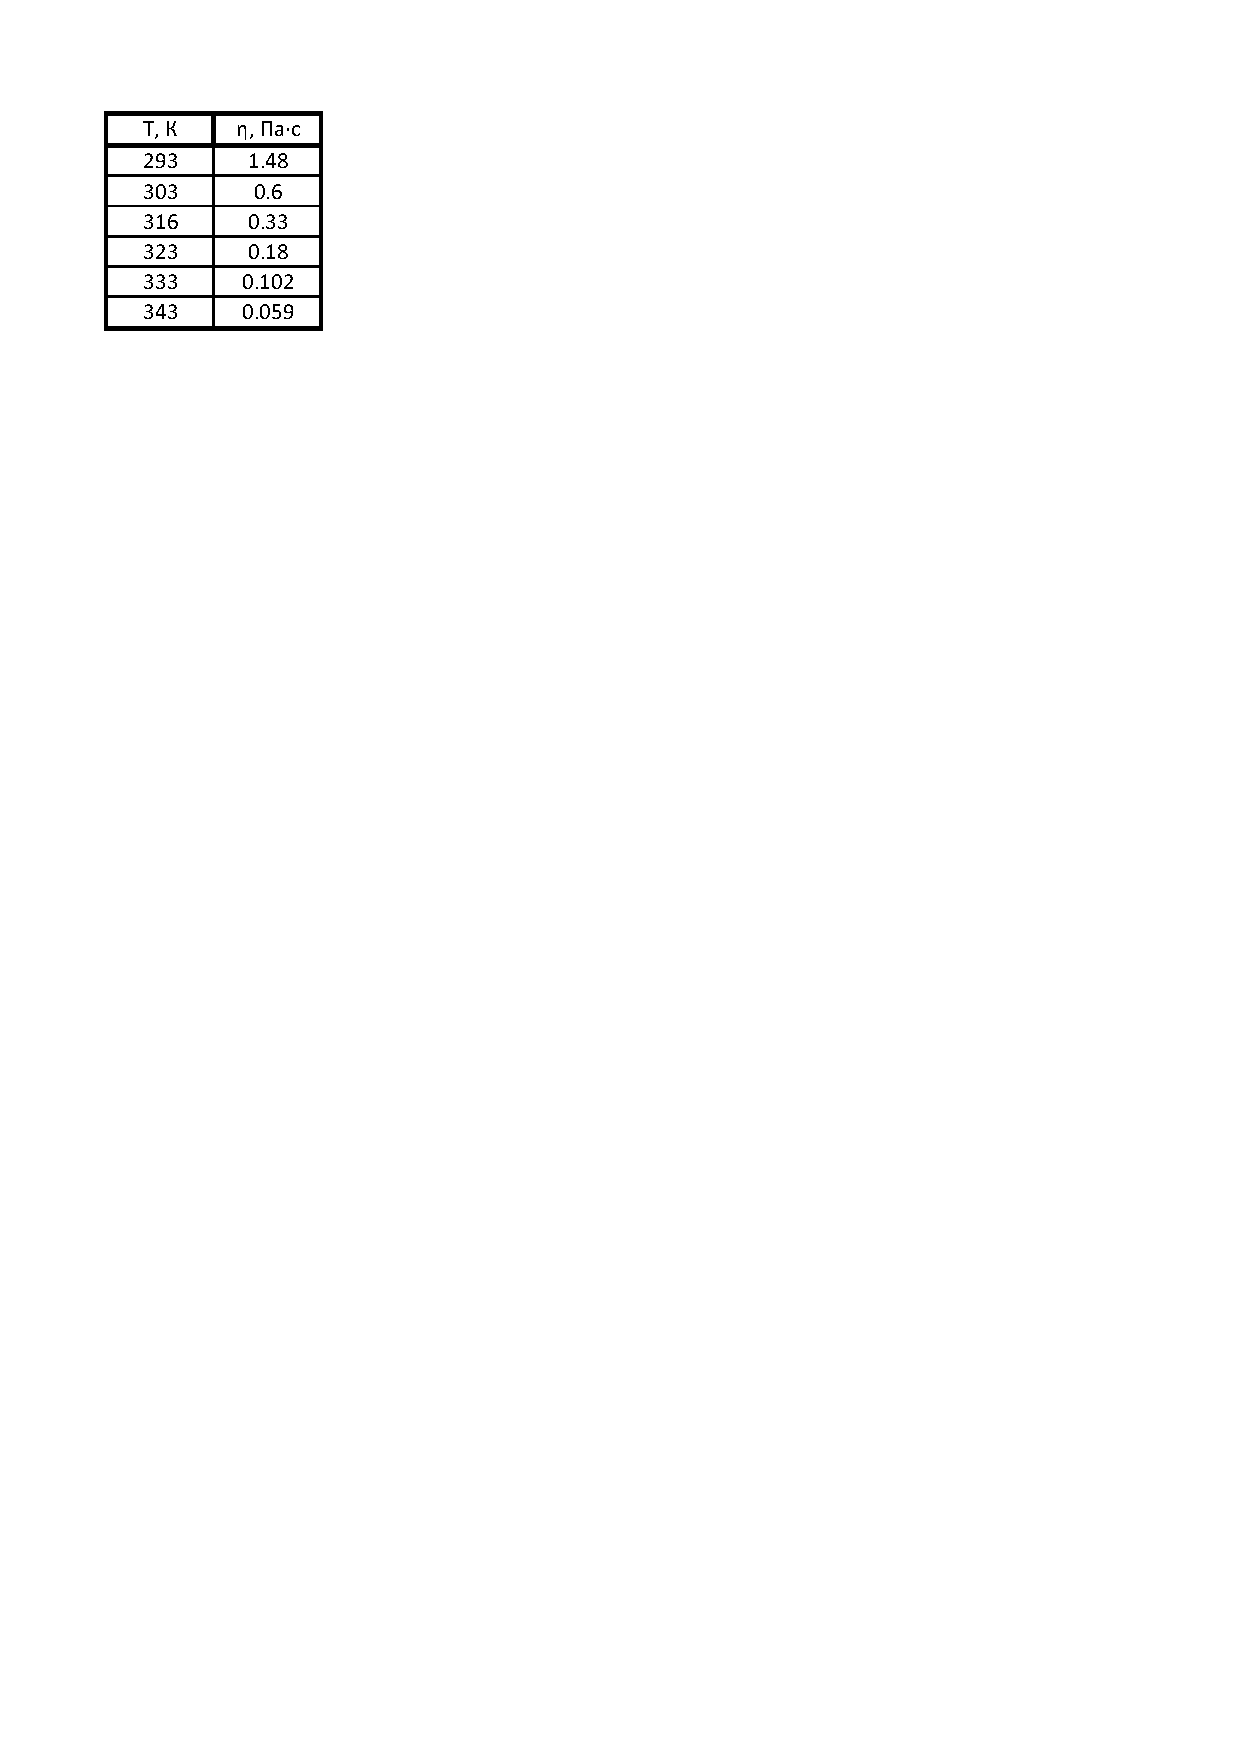
\includegraphics[height=0.2\textheight]{tabl_dann}\\
	\end{tabular}
	\caption{Табличные значения $\eta(T)$}
	\label{Tab:tab_dann}
\end{table}
откуда аналогично тому, что выполнялось в этой работе, можно получить значение энергии активации, равное:
$$
W = (0.55\pm 0.02) \text{ эВ},
$$
которое достаточно сильно отличается от полученного в работе (на 20\%). Это объясняется тем, что глицерин --- гигроскопичное вещество, и в нашем случае он не был абсолютно чистый. 



\section{Заключение}
В данной работе рассматривалось движение шарика в глицерине. 

После измерения скорости движения шарика, было получено значение энергии активации глицерина, равное $W = (0.458\pm0.005) \text{ эВ}$.

Это значение находится в допустимом согласовании с другими экспериментальными и табличными данными. 



\bibliography{mybibliography}
\bibliographystyle{gost705}

\end{document}
